% Options for packages loaded elsewhere
\PassOptionsToPackage{unicode}{hyperref}
\PassOptionsToPackage{hyphens}{url}
%
\documentclass[
]{book}
\usepackage{amsmath,amssymb}
\usepackage{iftex}
\ifPDFTeX
  \usepackage[T1]{fontenc}
  \usepackage[utf8]{inputenc}
  \usepackage{textcomp} % provide euro and other symbols
\else % if luatex or xetex
  \usepackage{unicode-math} % this also loads fontspec
  \defaultfontfeatures{Scale=MatchLowercase}
  \defaultfontfeatures[\rmfamily]{Ligatures=TeX,Scale=1}
\fi
\usepackage{lmodern}
\ifPDFTeX\else
  % xetex/luatex font selection
\fi
% Use upquote if available, for straight quotes in verbatim environments
\IfFileExists{upquote.sty}{\usepackage{upquote}}{}
\IfFileExists{microtype.sty}{% use microtype if available
  \usepackage[]{microtype}
  \UseMicrotypeSet[protrusion]{basicmath} % disable protrusion for tt fonts
}{}
\makeatletter
\@ifundefined{KOMAClassName}{% if non-KOMA class
  \IfFileExists{parskip.sty}{%
    \usepackage{parskip}
  }{% else
    \setlength{\parindent}{0pt}
    \setlength{\parskip}{6pt plus 2pt minus 1pt}}
}{% if KOMA class
  \KOMAoptions{parskip=half}}
\makeatother
\usepackage{xcolor}
\usepackage{color}
\usepackage{fancyvrb}
\newcommand{\VerbBar}{|}
\newcommand{\VERB}{\Verb[commandchars=\\\{\}]}
\DefineVerbatimEnvironment{Highlighting}{Verbatim}{commandchars=\\\{\}}
% Add ',fontsize=\small' for more characters per line
\usepackage{framed}
\definecolor{shadecolor}{RGB}{248,248,248}
\newenvironment{Shaded}{\begin{snugshade}}{\end{snugshade}}
\newcommand{\AlertTok}[1]{\textcolor[rgb]{0.94,0.16,0.16}{#1}}
\newcommand{\AnnotationTok}[1]{\textcolor[rgb]{0.56,0.35,0.01}{\textbf{\textit{#1}}}}
\newcommand{\AttributeTok}[1]{\textcolor[rgb]{0.13,0.29,0.53}{#1}}
\newcommand{\BaseNTok}[1]{\textcolor[rgb]{0.00,0.00,0.81}{#1}}
\newcommand{\BuiltInTok}[1]{#1}
\newcommand{\CharTok}[1]{\textcolor[rgb]{0.31,0.60,0.02}{#1}}
\newcommand{\CommentTok}[1]{\textcolor[rgb]{0.56,0.35,0.01}{\textit{#1}}}
\newcommand{\CommentVarTok}[1]{\textcolor[rgb]{0.56,0.35,0.01}{\textbf{\textit{#1}}}}
\newcommand{\ConstantTok}[1]{\textcolor[rgb]{0.56,0.35,0.01}{#1}}
\newcommand{\ControlFlowTok}[1]{\textcolor[rgb]{0.13,0.29,0.53}{\textbf{#1}}}
\newcommand{\DataTypeTok}[1]{\textcolor[rgb]{0.13,0.29,0.53}{#1}}
\newcommand{\DecValTok}[1]{\textcolor[rgb]{0.00,0.00,0.81}{#1}}
\newcommand{\DocumentationTok}[1]{\textcolor[rgb]{0.56,0.35,0.01}{\textbf{\textit{#1}}}}
\newcommand{\ErrorTok}[1]{\textcolor[rgb]{0.64,0.00,0.00}{\textbf{#1}}}
\newcommand{\ExtensionTok}[1]{#1}
\newcommand{\FloatTok}[1]{\textcolor[rgb]{0.00,0.00,0.81}{#1}}
\newcommand{\FunctionTok}[1]{\textcolor[rgb]{0.13,0.29,0.53}{\textbf{#1}}}
\newcommand{\ImportTok}[1]{#1}
\newcommand{\InformationTok}[1]{\textcolor[rgb]{0.56,0.35,0.01}{\textbf{\textit{#1}}}}
\newcommand{\KeywordTok}[1]{\textcolor[rgb]{0.13,0.29,0.53}{\textbf{#1}}}
\newcommand{\NormalTok}[1]{#1}
\newcommand{\OperatorTok}[1]{\textcolor[rgb]{0.81,0.36,0.00}{\textbf{#1}}}
\newcommand{\OtherTok}[1]{\textcolor[rgb]{0.56,0.35,0.01}{#1}}
\newcommand{\PreprocessorTok}[1]{\textcolor[rgb]{0.56,0.35,0.01}{\textit{#1}}}
\newcommand{\RegionMarkerTok}[1]{#1}
\newcommand{\SpecialCharTok}[1]{\textcolor[rgb]{0.81,0.36,0.00}{\textbf{#1}}}
\newcommand{\SpecialStringTok}[1]{\textcolor[rgb]{0.31,0.60,0.02}{#1}}
\newcommand{\StringTok}[1]{\textcolor[rgb]{0.31,0.60,0.02}{#1}}
\newcommand{\VariableTok}[1]{\textcolor[rgb]{0.00,0.00,0.00}{#1}}
\newcommand{\VerbatimStringTok}[1]{\textcolor[rgb]{0.31,0.60,0.02}{#1}}
\newcommand{\WarningTok}[1]{\textcolor[rgb]{0.56,0.35,0.01}{\textbf{\textit{#1}}}}
\usepackage{longtable,booktabs,array}
\usepackage{calc} % for calculating minipage widths
% Correct order of tables after \paragraph or \subparagraph
\usepackage{etoolbox}
\makeatletter
\patchcmd\longtable{\par}{\if@noskipsec\mbox{}\fi\par}{}{}
\makeatother
% Allow footnotes in longtable head/foot
\IfFileExists{footnotehyper.sty}{\usepackage{footnotehyper}}{\usepackage{footnote}}
\makesavenoteenv{longtable}
\usepackage{graphicx}
\makeatletter
\def\maxwidth{\ifdim\Gin@nat@width>\linewidth\linewidth\else\Gin@nat@width\fi}
\def\maxheight{\ifdim\Gin@nat@height>\textheight\textheight\else\Gin@nat@height\fi}
\makeatother
% Scale images if necessary, so that they will not overflow the page
% margins by default, and it is still possible to overwrite the defaults
% using explicit options in \includegraphics[width, height, ...]{}
\setkeys{Gin}{width=\maxwidth,height=\maxheight,keepaspectratio}
% Set default figure placement to htbp
\makeatletter
\def\fps@figure{htbp}
\makeatother
\setlength{\emergencystretch}{3em} % prevent overfull lines
\providecommand{\tightlist}{%
  \setlength{\itemsep}{0pt}\setlength{\parskip}{0pt}}
\setcounter{secnumdepth}{5}
\usepackage{booktabs}
\usepackage{amsthm}
\makeatletter
\def\thm@space@setup{%
  \thm@preskip=8pt plus 2pt minus 4pt
  \thm@postskip=\thm@preskip
}
\makeatother
\ifLuaTeX
  \usepackage{selnolig}  % disable illegal ligatures
\fi
\usepackage[]{natbib}
\bibliographystyle{apalike}
\usepackage{bookmark}
\IfFileExists{xurl.sty}{\usepackage{xurl}}{} % add URL line breaks if available
\urlstyle{same}
\hypersetup{
  pdftitle={EUR/USD},
  pdfauthor={Harvey Bastidas, Andrés Caicedo, Alexander Alvarado},
  hidelinks,
  pdfcreator={LaTeX via pandoc}}

\title{EUR/USD}
\author{Harvey Bastidas, Andrés Caicedo, Alexander Alvarado}
\date{2024-10-21}

\begin{document}
\maketitle

{
\setcounter{tocdepth}{1}
\tableofcontents
}
\chapter{Justificación de elección del Dataset}\label{justificaciuxf3n-de-elecciuxf3n-del-dataset}

\textbf{Integrantes}:\\
Harvey Bastidas, Alexander Alvarado y Andrés Caicedo\\
\textbf{Materia}:\\
Análisis de series de tiempo\\
\textbf{Profesora}:\\
Isabel Cristina García

\begin{center}\rule{0.5\linewidth}{0.5pt}\end{center}

\section{Información del Dataset}\label{informaciuxf3n-del-dataset}

El dataset seleccionado para este análisis es el siguiente: \href{https://www.kaggle.com/datasets/chandrimad31/eurusd-forex-trading-data-20032021}{EUR/USD Forex Trading Data (2003-2021)}, el cual fue extraído de \href{https://forex.tradingcharts.com/}{Forex Trading Charts}, propiedad de Barchart Solutions, una empresa especializada en servicios financieros en los Estados Unidos. Barchart Solutions cuenta con reconocidos clientes como el Banco Goldman Sachs y el Bank of Canada, lo que nos lleva a concluir que los datos ofrecidos son confiables y precisos para realizar análisis financieros.

La empresa matriz, \textbf{Barchart Solutions}, tiene su sede en:

\textbf{222 S. Riverside Plaza, Suite 810,\\
Chicago, IL 60606, Estados Unidos}

El dataset presenta las tasas de cambio del par de divisas EUR/USD desde el \textbf{5 de mayo de 2003} hasta el \textbf{16 de octubre de 2021}, con una periodicidad de \textbf{4 horas}. Este conjunto de datos incluye las siguientes 6 columnas:

\begin{itemize}
\tightlist
\item
  \textbf{Open}: Precio de apertura para el periodo.
\item
  \textbf{High}: Precio máximo durante el periodo.
\item
  \textbf{Low}: Precio mínimo durante el periodo.
\item
  \textbf{Close}: Precio de cierre para el periodo.
\item
  \textbf{Volume}: Volumen de transacciones reportado.
\end{itemize}

Es importante resaltar que los datos no contienen valores nulos ni perdidos para los días de semana, aunque no se registran valores durante los fines de semana, lo que es normal en los mercados de Forex.

El análisis se centrará en la columna \textbf{Close}, que representa el precio de cierre, dado que es la variable más relevante para el pronóstico de tendencias.

\section{Justificación de la Elección del Dataset}\label{justificaciuxf3n-de-la-elecciuxf3n-del-dataset}

La elección de este dataset se fundamenta en la importancia de analizar la tasa de cambio EUR/USD, uno de los pares de divisas más negociados en el mercado Forex. La predicción de la tendencia de la tasa de cambio es crucial para varias estrategias financieras, como el balanceo de portafolios de inversión. En este contexto, se pueden usar tanto la \textbf{Teoría Moderna de Portafolios (MPT)} como la \textbf{Teoría de Portafolios Post-Moderna (PMPT)}, que son ampliamente utilizadas en la optimización de la distribución de activos. Ambas teorías se benefician de predicciones precisas de la tendencia de los activos subyacentes, como es el caso de las divisas.

Además, este dataset ofrece una excelente relación señal-ruido, lo que mejora la predictibilidad de los modelos basados en series de tiempo. Utilizamos el \textbf{coeficiente de variación (CV)} como criterio para seleccionar este dataset, debido a que es una métrica robusta para medir la variabilidad en relación con la media. Un CV bajo indica que la variabilidad en los datos es relativamente baja, lo que es favorable para la predicción de tendencias.

El \textbf{coeficiente de variación} calculado para la columna ``Close'' de este dataset es de aproximadamente \textbf{9.5\%}, lo que lo convierte en el más bajo entre los datasets que evaluamos. Esto lo hace ideal para el pronóstico, ya que un CV bajo sugiere que la señal en los datos es fuerte en comparación con el ruido.

\subsection{Relación con el Signal-to-Noise Ratio (SNR)}\label{relaciuxf3n-con-el-signal-to-noise-ratio-snr}

El \textbf{coeficiente de variación (CV)} está inversamente relacionado con el \textbf{Signal-to-Noise Ratio (SNR)}, una métrica comúnmente utilizada en el procesamiento de señales. El SNR mide la proporción de la potencia de la señal con respecto a la del ruido, lo que ayuda a evaluar la calidad de los datos.

El SNR para este dataset se calcula como el cuadrado del inverso del CV. Para el EUR/USD, con un CV de \textbf{0.09}, el SNR es aproximadamente:

\[
SNR = \left(\frac{1}{0.09}\right)^2 \approx 123
\]

Este valor indica que la señal es mucho más fuerte que el ruido en este dataset. En contraste, otro dataset que probamos, con un CV de \textbf{20\%}, tenía un SNR mucho menor, alrededor de \textbf{25}. La diferencia muestra que el dataset de EUR/USD tiene una mayor preponderancia de señal sobre el ruido, lo que permite una mejor predictibilidad en los modelos de pronóstico.

Dado que sabemos que el \textbf{SNR} es aprox \textbf{123}, esto significa que el ruido es aprox 1/123 = \textbf{0.008} que nos da una idea del máximo error absoluto (\textbf{MAE}) en los datos Normalizados en el pronósitco del siguiente periodo que podemos obtener, ya que errores por debajo de este valor probablemente incluirían la predicción del ruido y podrían ser indicador de overfitting en el modelo predictivo usado.

\section{Importancia de Analizar este Dataset}\label{importancia-de-analizar-este-dataset}

La capacidad de predecir con precisión la tasa de cambio EUR/USD tiene múltiples aplicaciones en el sector financiero. En primer lugar, es fundamental para el \textbf{trading de divisas (Forex)}, donde una mejor predicción de las tendencias puede resultar en decisiones de inversión más acertadas. Además, es esencial para la gestión de portafolios financieros, ya que permite el uso de herramientas como la \textbf{Teoría Moderna de Portafolios (MPT)}, donde la diversificación se realiza teniendo en cuenta tanto la tendencia como la variabilidad de los activos.

Por lo tanto, este dataset fue seleccionado debido a su alta calidad y baja variabilidad, lo que lo hace ideal para el análisis predictivo en el mercado de Forex, así como en la gestión de portafolios. El alto \textbf{SNR} nos da confianza en que las predicciones basadas en este dataset serán precisas y útiles en un entorno real, al mismo tiempo que nos alerta sobre los límites predictivos en función del ruido presente en los datos.

\chapter{Estructura de los datos}\label{intro}

\section{Cálculo de Medias Móviles Simples:}\label{cuxe1lculo-de-medias-muxf3viles-simples}

\begin{Shaded}
\begin{Highlighting}[]
\CommentTok{\# Calcular las medias móviles}
\NormalTok{data}\SpecialCharTok{$}\NormalTok{MA\_short }\OtherTok{\textless{}{-}} \FunctionTok{SMA}\NormalTok{(data}\SpecialCharTok{$}\NormalTok{close, }\AttributeTok{n =} \DecValTok{50}\NormalTok{)  }\CommentTok{\# Media móvil de 50 periodos}
\NormalTok{data}\SpecialCharTok{$}\NormalTok{MA\_long }\OtherTok{\textless{}{-}} \FunctionTok{SMA}\NormalTok{(data}\SpecialCharTok{$}\NormalTok{close, }\AttributeTok{n =} \DecValTok{500}\NormalTok{)  }\CommentTok{\# Media móvil de 200 periodos}
\end{Highlighting}
\end{Shaded}

\begin{Shaded}
\begin{Highlighting}[]
\CommentTok{\# Eliminar filas con NA en las medias móviles}
\NormalTok{data\_clean }\OtherTok{\textless{}{-}} \FunctionTok{na.omit}\NormalTok{(data)}

\CommentTok{\# Crear el gráfico con las filas limpias}
\FunctionTok{ggplot}\NormalTok{(data\_clean, }\FunctionTok{aes}\NormalTok{(}\AttributeTok{x =} \FunctionTok{as.POSIXct}\NormalTok{(Gmt.time, }\AttributeTok{format =} \StringTok{"\%d.\%m.\%Y \%H:\%M:\%S"}\NormalTok{))) }\SpecialCharTok{+}
  \FunctionTok{geom\_line}\NormalTok{(}\FunctionTok{aes}\NormalTok{(}\AttributeTok{y =}\NormalTok{ close, }\AttributeTok{color =} \StringTok{"Close Price"}\NormalTok{)) }\SpecialCharTok{+}
  \FunctionTok{geom\_line}\NormalTok{(}\FunctionTok{aes}\NormalTok{(}\AttributeTok{y =}\NormalTok{ MA\_short, }\AttributeTok{color =} \StringTok{"50{-}period MA"}\NormalTok{)) }\SpecialCharTok{+}
  \FunctionTok{geom\_line}\NormalTok{(}\FunctionTok{aes}\NormalTok{(}\AttributeTok{y =}\NormalTok{ MA\_long, }\AttributeTok{color =} \StringTok{"500{-}period MA"}\NormalTok{)) }\SpecialCharTok{+}
  \FunctionTok{labs}\NormalTok{(}\AttributeTok{title =} \StringTok{"EUR/USD Close Price with Moving Averages"}\NormalTok{,}
       \AttributeTok{x =} \StringTok{"Date"}\NormalTok{, }\AttributeTok{y =} \StringTok{"Price"}\NormalTok{) }\SpecialCharTok{+}
  \FunctionTok{scale\_color\_manual}\NormalTok{(}\AttributeTok{values =} \FunctionTok{c}\NormalTok{(}\StringTok{"Close Price"} \OtherTok{=} \StringTok{"black"}\NormalTok{, }
                                \StringTok{"50{-}period MA"} \OtherTok{=} \StringTok{"blue"}\NormalTok{, }
                                \StringTok{"500{-}period MA"} \OtherTok{=} \StringTok{"red"}\NormalTok{)) }\SpecialCharTok{+}
  \FunctionTok{theme\_minimal}\NormalTok{()}
\end{Highlighting}
\end{Shaded}

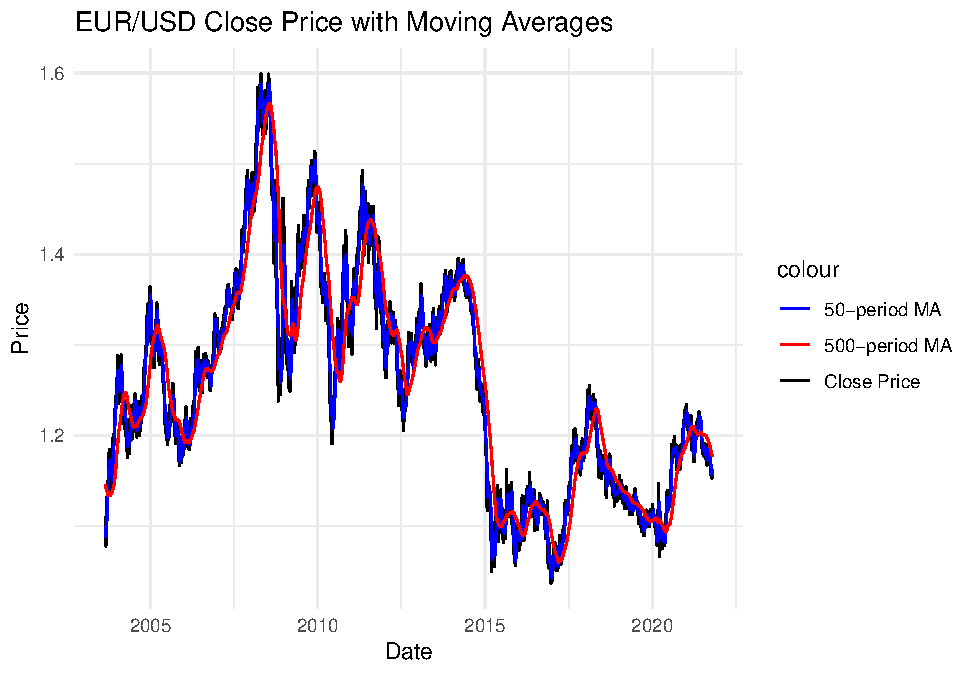
\includegraphics{bookdown_time_series_files/figure-latex/unnamed-chunk-3-1.pdf}

\section{Análisis de Rezagos}\label{anuxe1lisis-de-rezagos}

Cómo se comporta la serie de tiempo con respecto a sus valores pasados, introduciendo rezagos.

\begin{Shaded}
\begin{Highlighting}[]
\CommentTok{\# Crear la serie de tiempo con frecuencia de 6 (observaciones diarias)}
\NormalTok{ts\_close }\OtherTok{\textless{}{-}} \FunctionTok{ts}\NormalTok{(data}\SpecialCharTok{$}\NormalTok{close, }\AttributeTok{frequency =} \DecValTok{6}\NormalTok{)  }\CommentTok{\# 6 periodos por día}
\end{Highlighting}
\end{Shaded}

\begin{Shaded}
\begin{Highlighting}[]
\CommentTok{\# Visualizar los rezagos con lag.plot}
\FunctionTok{lag.plot}\NormalTok{(ts\_close, }\AttributeTok{lags =} \DecValTok{9}\NormalTok{, }\AttributeTok{layout =} \FunctionTok{c}\NormalTok{(}\DecValTok{3}\NormalTok{, }\DecValTok{3}\NormalTok{), }\AttributeTok{main =} \StringTok{"Lag Plots of Close Prices (4{-}Hour Intervals)"}\NormalTok{)}
\end{Highlighting}
\end{Shaded}

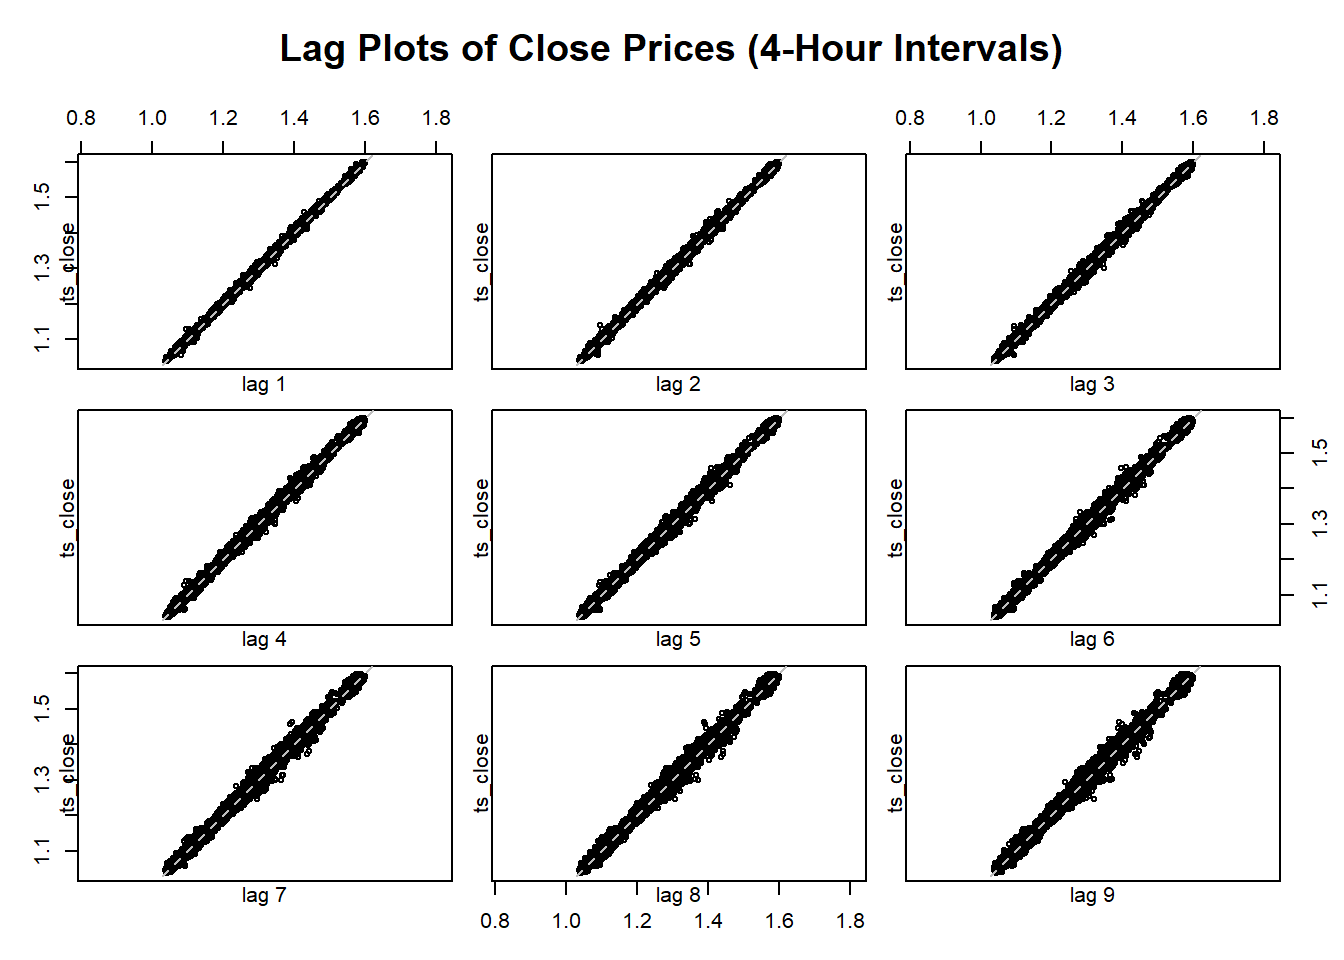
\includegraphics{bookdown_time_series_files/figure-latex/unnamed-chunk-5-1.pdf}

En cada uno de los gráficos, los puntos siguen una línea casi perfectamente recta, sugiriendo una \textbf{alta autocorrelación} entre los valores de la serie con sus rezagos cercanos.

La pendiente positiva indica que cuando el valor anterior era alto, el valor actual también tiende a ser alto, y lo mismo sucede para valores bajos. Esto sugiere que \textbf{la serie es muy persistente}, es decir, los precios tienden a seguir una dirección similar en el corto plazo.

Dado que no hay patrones dispersos o sin forma definida, se puede inferir que la serie no tiene cambios abruptos o comportamiento caótico entre los puntos cercanos. Esto podría indicar que \textbf{no hay mucha volatilidad} en los intervalos de 4 horas.

\section{Análisis de Estacionalidad}\label{anuxe1lisis-de-estacionalidad}

Para detectar si existe estacionalidad (patrones repetitivos), utilizaremos \textbf{decomposición} o \textbf{test de estacionalidad}.

\begin{Shaded}
\begin{Highlighting}[]
\FunctionTok{library}\NormalTok{(forecast)}
\end{Highlighting}
\end{Shaded}

\begin{verbatim}
## Warning: package 'forecast' was built under R version 4.3.3
\end{verbatim}

\begin{verbatim}
## Registered S3 method overwritten by 'quantmod':
##   method            from
##   as.zoo.data.frame zoo
\end{verbatim}

\begin{Shaded}
\begin{Highlighting}[]
\CommentTok{\# Convertir los datos a una serie de tiempo (asumiendo que son horarios)}
\NormalTok{ts\_data }\OtherTok{\textless{}{-}} \FunctionTok{ts}\NormalTok{(data}\SpecialCharTok{$}\NormalTok{close, }\AttributeTok{frequency =} \DecValTok{24} \SpecialCharTok{*} \DecValTok{30}\NormalTok{)  }\CommentTok{\# 24 datos diarios, 30 días al mes}

\CommentTok{\# Descomposición STL}
\NormalTok{decomposed }\OtherTok{\textless{}{-}} \FunctionTok{stl}\NormalTok{(ts\_data, }\AttributeTok{s.window =} \StringTok{"periodic"}\NormalTok{)}

\CommentTok{\# Graficar la descomposición}
\FunctionTok{plot}\NormalTok{(decomposed)}
\end{Highlighting}
\end{Shaded}

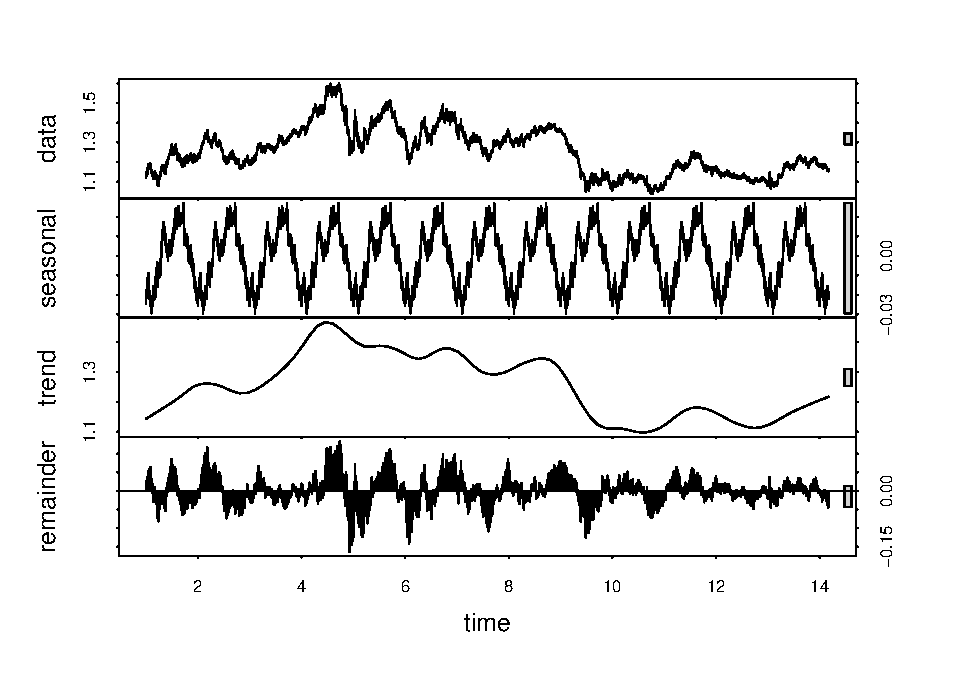
\includegraphics{bookdown_time_series_files/figure-latex/unnamed-chunk-6-1.pdf}

En la gráfica de \textbf{descomposición de series de tiempo} que muestras, se visualizan los \textbf{componentes de la serie}: datos originales, estacionalidad, tendencia y residuales (remainder). A continuación, te explico cómo interpretar cada componente:

\subsection{\texorpdfstring{1. \textbf{Datos Originales (data)}}{1. Datos Originales (data)}}\label{datos-originales-data}

\begin{itemize}
\item
  En la primera gráfica (data), se observan los valores de cierre a lo largo del tiempo.
\item
  Vemos fluctuaciones en los precios con algunas subidas y bajadas claras, lo que indica la volatilidad normal del mercado Forex.
\end{itemize}

\subsection{\texorpdfstring{2. \textbf{Componente Estacional (seasonal)}}{2. Componente Estacional (seasonal)}}\label{componente-estacional-seasonal}

\begin{itemize}
\item
  El segundo gráfico muestra un \textbf{patrón repetitivo y periódico}. Este patrón sugiere que hay \textbf{ciclos regulares} en la serie.
\item
  La estacionalidad se mantiene constante a lo largo del tiempo, lo que indica que ciertos movimientos en el mercado se repiten con una periodicidad fija (en este caso, podría ser diaria o semanal).
\end{itemize}

\textbf{Interpretación}:

\begin{itemize}
\item
  \textbf{Mercados Forex} suelen tener patrones intradía o semanales, influenciados por la apertura y cierre de mercados (como los de Nueva York, Londres y Tokio).
\item
  Es probable que este componente estacional refleje la actividad cíclica en horarios específicos o días determinados, como mayor volatilidad durante sesiones overlap (como entre Londres y Nueva York).
\end{itemize}

\subsection{\texorpdfstring{3. \textbf{Componente de Tendencia (trend)}}{3. Componente de Tendencia (trend)}}\label{componente-de-tendencia-trend}

\begin{itemize}
\item
  El tercer gráfico muestra una \textbf{tendencia suavizada} que sigue la dirección general del mercado.
\item
  Observamos fases de \textbf{alzas y caídas}: primero hay una subida clara, luego una caída, y finalmente otra leve tendencia hacia la estabilidad.
\end{itemize}

\textbf{Interpretación}:

\begin{itemize}
\tightlist
\item
  Este componente captura el \textbf{movimiento de largo plazo} del mercado. Aquí, parece que el mercado tiene ciclos de crecimiento seguidos de correcciones, algo común en activos como las divisas.
\end{itemize}

\subsection{\texorpdfstring{4. \textbf{Componente de Residuos o Resto (remainder)}}{4. Componente de Residuos o Resto (remainder)}}\label{componente-de-residuos-o-resto-remainder}

\begin{itemize}
\item
  El último gráfico (remainder) muestra los \textbf{residuos} o la parte de los datos que no es explicada por la tendencia ni la estacionalidad.
\item
  Estos residuos parecen ser \textbf{ruido blanco}, con fluctuaciones alrededor de cero, lo que indica que no hay patrones significativos adicionales no capturados por los otros componentes.
\end{itemize}

\textbf{Interpretación}:

\begin{itemize}
\tightlist
\item
  Un buen modelo de descomposición debe dejar los residuos sin patrones claros, como sucede en este caso. Esto indica que la tendencia y la estacionalidad explican bien el comportamiento de la serie.
\end{itemize}

Prueba de estacionalidad con adf.test:

\begin{Shaded}
\begin{Highlighting}[]
\FunctionTok{library}\NormalTok{(tseries)}
\end{Highlighting}
\end{Shaded}

\begin{verbatim}
## Warning: package 'tseries' was built under R version 4.3.3
\end{verbatim}

\begin{Shaded}
\begin{Highlighting}[]
\CommentTok{\# Prueba de Dickey{-}Fuller aumentada para detectar estacionalidad}
\NormalTok{adf\_test }\OtherTok{\textless{}{-}} \FunctionTok{adf.test}\NormalTok{(ts\_data, }\AttributeTok{alternative =} \StringTok{"stationary"}\NormalTok{)}
\FunctionTok{print}\NormalTok{(adf\_test)}
\end{Highlighting}
\end{Shaded}

\begin{verbatim}
## 
##  Augmented Dickey-Fuller Test
## 
## data:  ts_data
## Dickey-Fuller = -2.8283, Lag order = 30, p-value = 0.2269
## alternative hypothesis: stationary
\end{verbatim}

  \bibliography{book.bib,packages.bib}

\end{document}
